\usepackage{graphicx}
\usepackage{float}
\chapter{Grandes modelos de lenguaje}
\chapterauthor{Alejandro Silva Rodríguez}

\definecolor{codegreen}{HTML}{5AB2FF}
\definecolor{morado}{HTML}{AD88C6}
\definecolor{BG}{HTML}{EEEEEE}
\definecolor{azul}{HTML}{4D869C}
\lstdefinestyle{mystyle}{
    language=Python,
    backgroundcolor=\color{BG},
    commentstyle=\color{codegreen},
    basicstyle=\ttfamily\small,
    keywordstyle=\color{azul},
    commentstyle=\color{codegreen},
    stringstyle=\color{morado},
    showstringspaces=false,
    breaklines=true,
    frame=shadowbox,
    numbers=left,
    numberstyle=\tiny\color{gray},
    captionpos=b,
}


\section{Introducción}
Los grandes modelos de lenguaje (LLM) son una categoría de modelos avanzados entrenados con enormes conjuntos de datos para comprender y generar lenguaje natural y otros tipos de contenido, permitiendo una amplia gama de aplicaciones.\\

Estos modelos se han vuelto mundialmente conocidos al llevar la IA generativa al centro de atención pública y empresarial. Aunque parecen recientes para algunos, empresas como IBM han estado implementándolos durante años para mejorar las capacidades de comprensión y procesamiento del lenguaje natural (NLU y NLP), aprovechando avances en aprendizaje automático, algoritmos y redes neuronales.\\

Los LLM representan un avance crucial en PLN y IA, siendo accesibles a través de interfaces como ChatGPT-3 y GPT-4 de OpenAI, Meta's Llama, y modelos de Google como BERT/RoBERTa y PaLM.  Estos modelos están diseñados para comprender y generar texto como humanos, basándose en datos masivos. Pueden traducir, resumir, responder preguntas, ayudar en tareas creativas y más, gracias a sus miles de millones de parámetros. Estos modelos avanzados pueden nutrirse de enormes cantidades de datos, incluyendo registros de Internet como Common Crawl, con más de 50 mil millones de páginas web, y Wikipedia, que cuenta con alrededor de 57 millones de páginas.\cite{IBM-LLM}\\

Los LLM están transformando aplicaciones como chatbots, asistentes virtuales, generación de contenido y más. Evolucionarán continuamente, remodelando nuestra interacción con la tecnología y el acceso a la información en el mundo digital moderno.


\section{Composición de Modelos de Lenguaje Grandes}

\subsection{Antecedentes}

Antes de la llegada de los Transformers, los modelos de lenguaje basados en redes neuronales recurrentes (RNN) eran dominantes en tareas de procesamiento de lenguaje natural (NLP). Estos modelos, como las RNN y las variantes como las LSTM (Long Short-Term Memory) y las GRU (Gated Recurrent Units), tenían la capacidad de procesar secuencias de datos, como palabras o caracteres, de manera progresiva, manteniendo una especie de "memoria" de los pasos anteriores.\cite{IBM-RNN}

Sin embargo, los modelos basados en RNN tenían varias limitaciones:
\begin{enumerate}
    
\item Problema de desvanecimiento/exploración del gradiente: Durante el entrenamiento, los gradientes (que indican cómo deben actualizarse los pesos de la red) pueden volverse muy pequeños o muy grandes a medida que se propagan hacia atrás a través de las capas de la red recurrente. Esto puede hacer que los modelos olviden información a largo plazo o que se vuelvan inestables (explosión del gradiente).
\item Ineficiencia en paralelización: Debido a su naturaleza secuencial(Figura \ref{fig:rnn}), las RNN no pueden procesar múltiples partes de una secuencia simultáneamente, lo que limita su capacidad para aprovechar el paralelismo y, por lo tanto, su eficiencia computacional.
\item Incapacidad para capturar relaciones a largo plazo: A pesar de las variantes como las LSTM y las GRU, las RNN todavía tenían dificultades para capturar dependencias a largo plazo en secuencias de datos, lo que limitaba su capacidad para comprender contextos complejos en tareas de NLP.
\item Costo computacional y tiempo de entrenamiento: Entrenar modelos basados en RNN puede ser computacionalmente costoso y llevar mucho tiempo, especialmente cuando se trabaja con grandes conjuntos de datos y arquitecturas complejas.
\end{enumerate}

\begin{figure}[H]
    \centering
    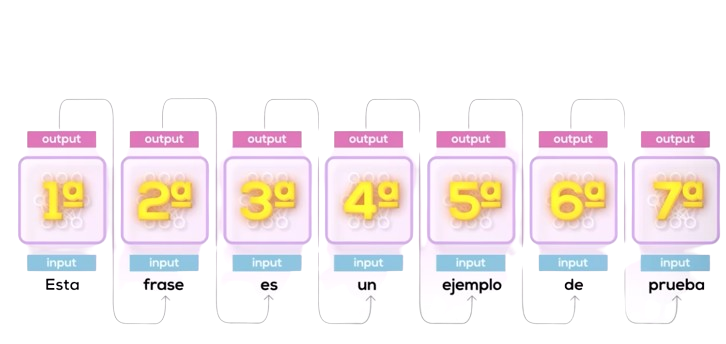
\includegraphics[width=0.6\textwidth]{plantilla-libro/img/rnn.png}
    \caption{RNN Procesando oración. Fuente: \cite{video-youtube}}
    \label{fig:rnn}
\end{figure}

El salto a los Transformers se dio principalmente debido a la introducción de la arquitectura de atención. Los Transformers abordan muchas de las limitaciones de las RNN:
\begin{enumerate}

\item Atención: Los Transformers utilizan mecanismos de atención que les permiten procesar palabras en paralelo en lugar de secuencialmente, lo que mejora significativamente la eficiencia y la capacidad de capturar relaciones a largo plazo.
\item Paralelización completa: Gracias a la atención y a la estructura basada en autoatención, los Transformers pueden paralelizar completamente el cálculo en todas las posiciones de la secuencia, lo que acelera tanto el entrenamiento como la inferencia.
\end{enumerate}








\subsection{Transtofmer}
Un transformer se compone de dos partes principales, encoder y decoder, cuyos componentes profundaremos más adelante:

 El encoder toma una secuencia de entrada y la transforma en vectores de representación, capturando las relaciones entre las palabras mediante capas de autoatención. Su objetivo principal es procesar la información de entrada y generar representaciones vectoriales contextualizadas que contienen información sobre cada elemento de la secuencia. Por otro lado, el decoder utiliza estos vectores de representación generados por el encoder, junto con la información condicional, para generar una secuencia de salida. También utiliza capas de autoatención, pero su enfoque se centra en capturar las relaciones entre las palabras en la secuencia de salida. Su función principal es generar una secuencia de salida coherente basada en la información proporcionada por el encoder y en los tokens previamente generados.

 La primera fase a la que se someten los datos al entrar a un transformer es la tokerización

 \subsubsection{Embeddings (Incrustaciones)}
   Los embeddings son representaciones vectoriales de palabras o tokens en un espacio dimensional(Figura \ref{fig:embedding}). En el contexto de los LLM, las embeddings se utilizan para transformar las palabras o tokens del vocabulario en vectores numéricos densos. Estos vectores capturan relaciones semánticas y sintácticas entre las palabras, lo que ayuda al modelo a aprender patrones y generalizar mejor sobre el lenguaje.

\begin{quote}
'Embedding aims at creating a vector representation of words. Words that have the same meaning will be close in terms of euclidian distance. For example, the word bathroomand shower are associated with the same concept, so we can see that the two words are close in Euclidean space, they express similar senses or concept.'\cite{atention-blog}

\end{quote}
   
   \begin{figure}[H]
        \centering
        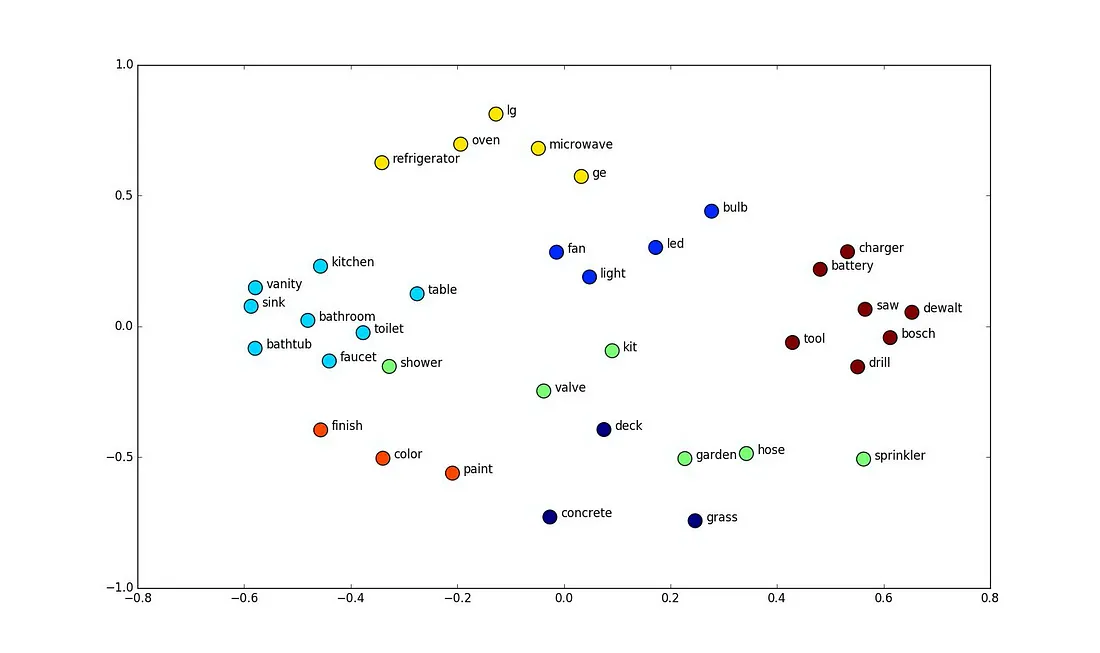
\includegraphics[width=.45\textwidth]{plantilla-libro/img/espacio_vectorial_encoding.png}
        \caption{Embedding vector representation of words. Fuente: \cite{atention-blog}}
        \label{fig:embedding}
    \end{figure}

 \newpage
 \subsubsection{Positional Encoding}
 Justo despues de esto, las palabras se pasan por un positional encoding, que le añade al token información sobre la posición de la palabra.
    En esencia, el positional encoding asigna un vector único a cada posición en la secuencia, de modo que palabras o elementos que ocupan posiciones diferentes tendrán representaciones distintas en el espacio vectorial, a pesar de que sus características semánticas sean similares.
    Se utiliza para abordar la falta de información sobre la posición en modelos como los transformers, donde la entrada se representa mediante embeddings que no contienen información sobre la ubicación de los tokens en la secuencia. Anteriormente, los modelos recurrentes obtenian información de la posicion de las palabras mediante la iteración en el texto, esta etapa fue la revolucionaría que propulsó el avance de los transformers.
\subsubsection{Capas de Atención (Attention Layers)}

   Las capas de atención son componentes clave dentro de los transformadores. Permiten que el modelo "preste atención" a diferentes partes de la secuencia de entrada durante el procesamiento. Esta atención se calcula dinámicamente para cada par de elementos en la secuencia, lo que ayuda al modelo a capturar relaciones contextuales y a decidir qué partes de la entrada son más relevantes para la tarea en cuestión.
\begin{figure}[H]
\begin{minipage}[f]{0.5\textwidth}
  \centering
  Scaled Dot-Product Attention \\
  \vspace{0.5cm}
  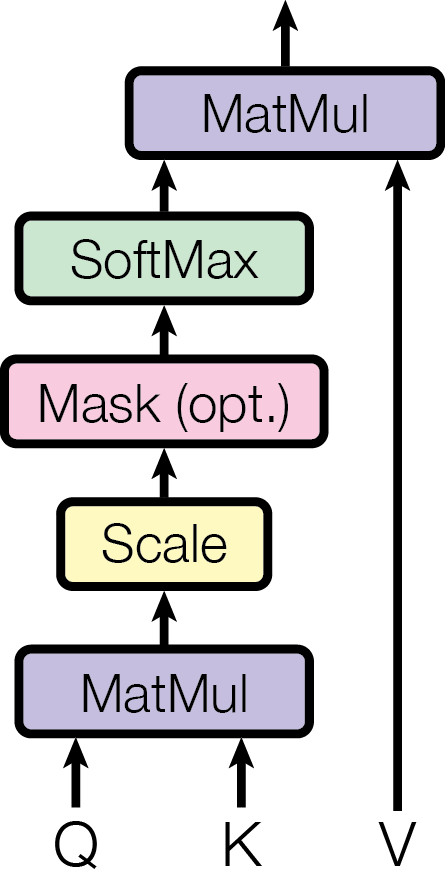
\includegraphics[scale=0.6]{plantilla-libro/ModalNet-19.png}
\end{minipage}
\begin{minipage}[f]{0.5\textwidth}
  \centering 
  Multi-Head Attention \\
  \vspace{0.1cm}
  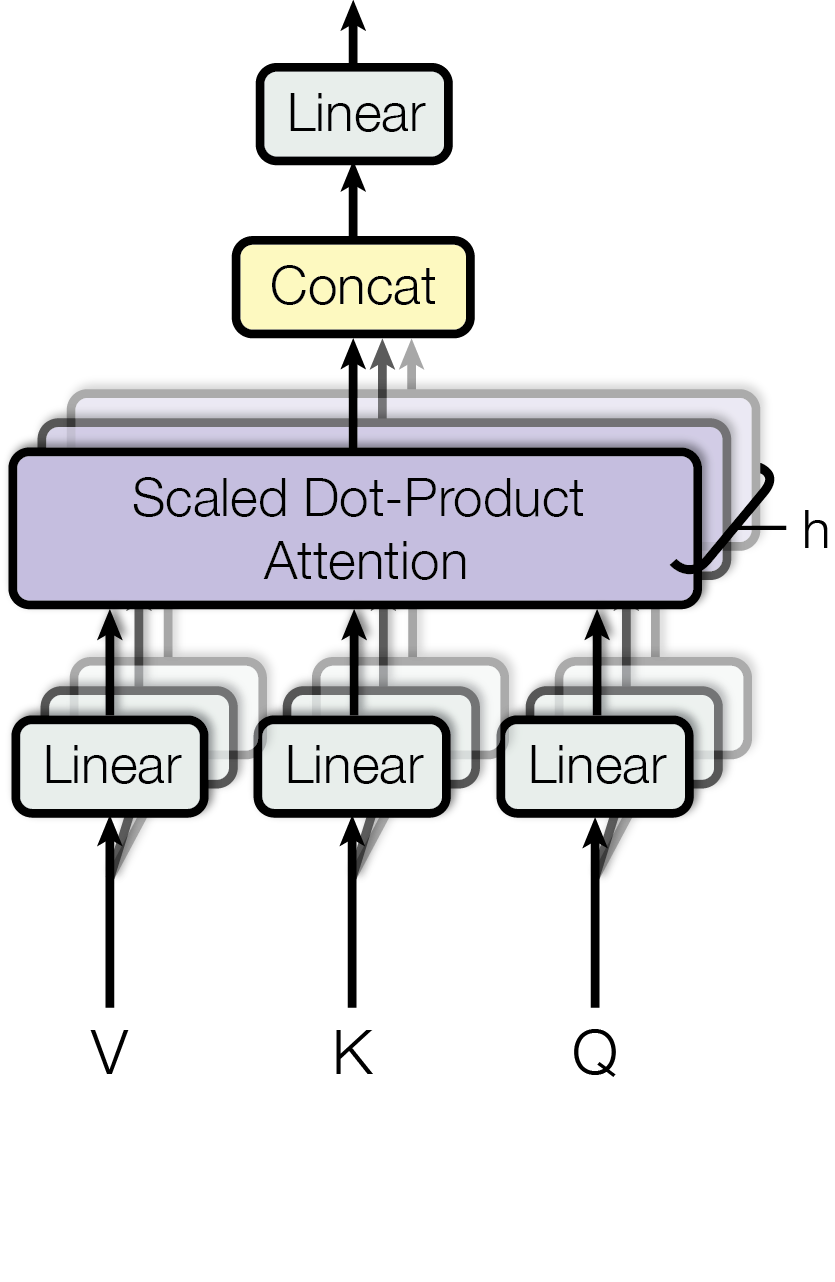
\includegraphics[scale=0.6]{plantilla-libro/ModalNet-20.png}  
\end{minipage}


  % \centering

  \caption{(izquierda) Scaled Dot-Product Attention. (derecha) Multi-Head Attention consists of several attention layers running in parallel. Fuente: \cite{vaswani2023attention}}
  \label{fig:multi-head-att}
\end{figure}
\newpage
El proceso comienza con tres conjuntos de vectores: consultas, claves y valores(Figura~\ref{fig:multi-head-att}). Por así decirlo, el vector clave sera un identificador que describe las propiedades de una palabra, mientras que el vector consulta describe las propiedades que busca una palabra. Estos vectores se derivan de la entrada original y se utilizan para calcular la atención. Primero, se calcula la similitud entre la consulta y cada clave utilizando el producto escalar obteniendo el vector  de atención, y luego se aplica una función softmax para obtener pesos de atención normalizados. Estos pesos determinan cuánta atención se asigna a cada valor correspondiente. Finalmente, se calcula una combinación lineal ponderada de los valores utilizando los pesos de atención, produciendo así la salida de la capa de atención. \cite{video-youtube}

El resultado será de alguna forma a que palabras muestra atención cuando se fija en una, dando una capacidad extraordinaria para reconocer el contexto. 

   
   \begin{figure}[h]
       \centering
       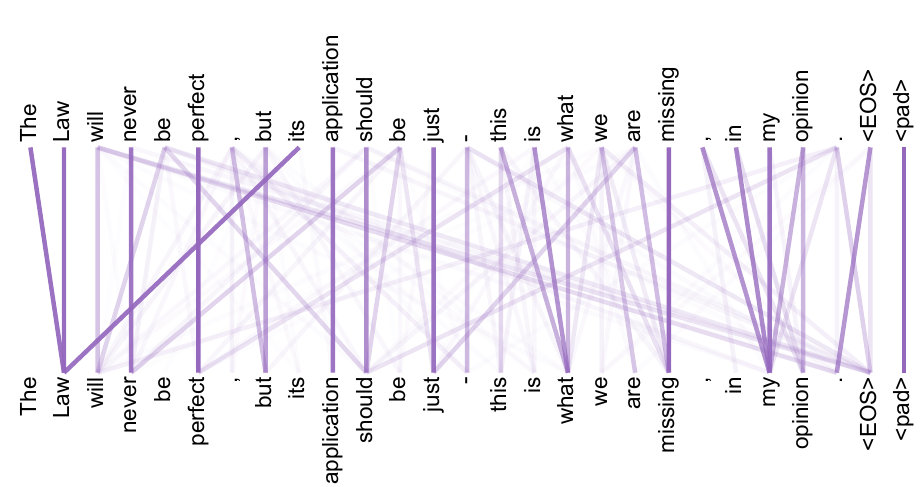
\includegraphics[width=.7\textwidth]{plantilla-libro/img/clave_valor_atencion.png}
       \caption{Representación del mecanismo de atención. Fuente: \cite{vaswani2023attention}}
       \label{fig:representacon_atencion}
   \end{figure}
    Ejemplo(Figura \ref{fig:representacon_atencion}):
    
    The law will never be perfect, but its application should be just.
    
    Cuando el modelo está procesando la secuencia, ¿a qué se refiere «its»? Parece una pregunta muy sencilla para una persona, pero se trata de un problema complejo que ha existido durante bastante tiempo en NLP. El mecanismo de auto-atención permite asociar «its» con Law en vez de con el resto de palabras.
    

\newpage
    \begin{figure}[H]
            \centering
            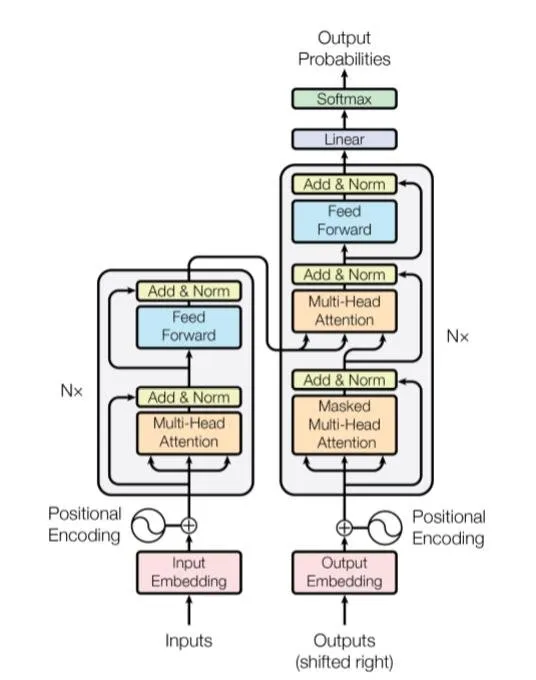
\includegraphics[width=.6\textwidth]{plantilla-libro/img/transformer_architecture.png}
            \caption{Transformer Architecture. Fuente: \cite{vaswani2023attention}}
            \label{fig:transformer}
        \end{figure}
    \subsubsection{Flujo de datos}
    Para resumir y ver como encajan todos los componentes analizaremos el flujo de datos en un transformer. 
    Primero, la palabra input es transformada en vector con información semantica y de posicion. A continuación entra en el encoder(Figura \ref{fig:transformer} parte de la izquierda) donde se extrae información de contexto mediante la atención, generando un output.
    En la segunda etapa, en el decoder(Figura \ref{fig:transformer} parte de la derecha), la multi-head attention layer es alimentada con el output del encoder, además de utilizar el output de una interación anterior como input. 
    Al final, estos dos componentes trabajarán juntos para predecir la palabra con mayor probabilidad de todo el vocabulario apoyado de una capa Softmax y One-hot Encoding.\cite{atention-blog}
\subsection{Arquitecturas más importantes}
\subsubsection{Generative Pre-trained Transformer (GPT)}
     
     Es un modelo de lenguaje desarrollado por OpenAI basado en la arquitectura Transformer. GPT utiliza una estructura unidireccional en la que las capas Transformer procesan la secuencia de entrada en una dirección. Cada bloque Transformer en GPT consta de capas de atención multi-cabeza seguidas de redes neuronales feedforward(Figura \ref{fig:gpt}). Es un modelo autoregresivo que genera texto palabra por palabra utilizando un token especial de inicio y predice la siguiente palabra en la secuencia. GPT se destaca en tareas de generación de texto y comprensión del lenguaje natural.
     Método de aprendizage:
     \begin{itemize}
         \item En el método autoregresivo, el modelo genera secuencialmente cada token de salida basado en los tokens previamente generados en la secuencia. Este enfoque busca maximizar la probabilidad conjunta de predecir cada token dado el contexto anterior.

     \end{itemize}
    'GPT-3 has 175 billion parameters, almost 2,000 times more than the number of parameters in the original GPT-1 model and over 100 times more than the 1.5 billion parameters in GPT-2.'\cite{gpt}
    \begin{figure}[h]
        \centering
        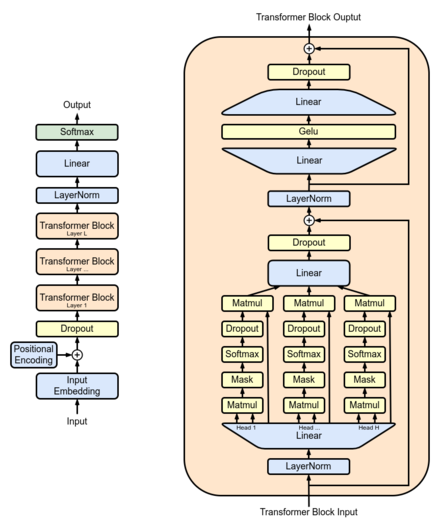
\includegraphics[width=0.55\textwidth]{plantilla-libro/img/gpt_architecture.png}
        \caption{GPT Architecture. Fuente: \cite{gpt-architecture}}
        \label{fig:gpt}
    \end{figure}
\newpage
\subsubsection{Bidirectional Encoder Representations from Transformers(BERT)}

    Desarrollado por Google, es otro modelo basado en la arquitectura Transformer. A diferencia de GPT, BERT utiliza un codificador bidireccional que procesa la secuencia de entrada en ambas direcciones, capturando así mejor el contexto bidireccional de las palabras. BERT se pre-entrena en tareas de Masked Language Modeling (MLM) y Next Sentence Prediction (NSP) (Figura \ref{fig:bert}), lo que le permite aprender representaciones contextuales profundas. Aunque BERT no es autoregresivo y no se utiliza directamente para la generación de texto, se utiliza ampliamente como modelo de representación contextual en tareas de procesamiento del lenguaje natural como clasificación de texto, extracción de información y más. BERT ha demostrado ser muy efectivo en la captura de relaciones semánticas y sintácticas en el texto.\cite{devlin2019bert}

    Metodos de aprendizage:
    \begin{itemize}
        \item Masked Language Modeling (MLM), se enmascaran aleatoriamente algunas palabras en las oraciones de entrada y el modelo debe predecir las palabras enmascaradas basándose en el contexto. Este método fomenta a BERT a entender el contexto de las palabras en relación con las demás en la oración.   
        \item Next Sentence Prediction (NSP) implica alimentar a BERT con pares de oraciones y el modelo debe predecir si la segunda oración sigue a la primera en el texto original. Esto ayuda a BERT a captar la coherencia entre las oraciones y entender la relación entre ellas. Ambos métodos son clave en el pre-entrenamiento de BERT para capturar información contextual y semántica en el texto.
    \end{itemize}
    \begin{figure}[h]
        \centering
        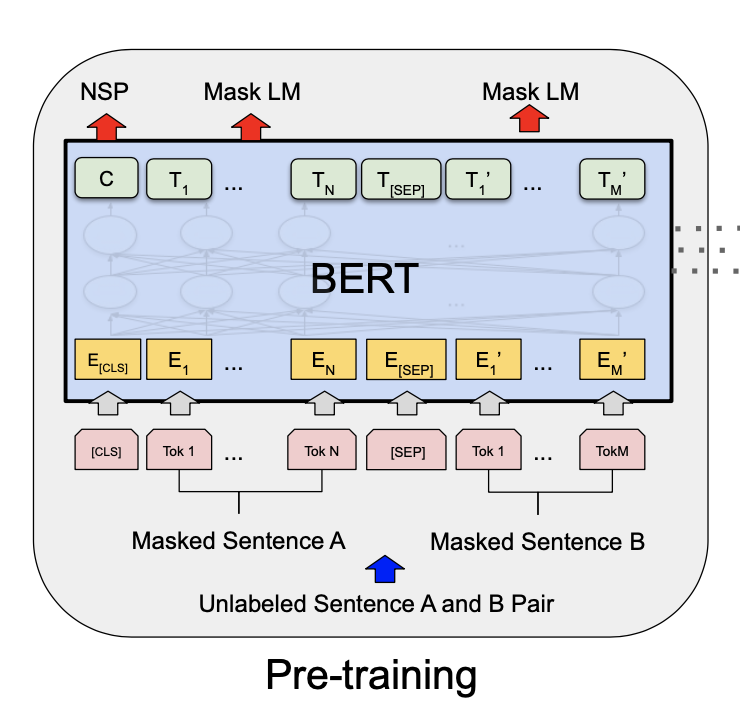
\includegraphics[width=0.6\textwidth]{plantilla-libro/img/bert_architecture.png}
        \caption{Bert Architecture. Fuente: \cite{devlin2019bert}}
        \label{fig:bert}
    \end{figure}
\newpage

\subsection{Pre-entrenamiento}
 Comienza con la recopilación de enormes cantidades de texto de diversas fuentes, que pueden incluir libros, artículos en línea, redes sociales y más. Este corpus de texto se utiliza para entrenar el modelo de forma no supervisada, lo que significa que el modelo aprende patrones y estructuras del lenguaje sin la necesidad de etiquetas o supervisión explícita. Antes de entrenar, el texto se tokeniza y preprocesa para convertirlo en unidades de entrada comprensibles para el modelo. Durante el entrenamiento, el modelo ajusta sus pesos para predecir palabras o partes de palabras en función del contexto proporcionado por la secuencia de tokens de entrada.




\section{Aplicaciones de Modelos de Lenguaje Grandes}
\subsection{Generación de Texto}
Ejemplos de generación de texto coherente y creativo incluyen la capacidad de los modelos de lenguaje grandes para producir artículos, historias, poemas y respuestas humanizadas. Estas aplicaciones son fundamentales en asistentes virtuales como Siri, chatbots como ChatGPT, y herramientas de escritura asistida que pueden generar contenido automáticamente.

\subsection{Clasificación de Texto}
Los modelos de lenguaje grandes se utilizan ampliamente en tareas de clasificación de texto, como análisis de sentimientos (determinar emociones en textos), detección de spam (identificación de mensajes no deseados), y categorización de noticias o documentos. Estos modelos pre-entrenados se benefician del transfer learning, permitiendo adaptarlos eficazmente a tareas específicas con datos de entrenamiento adicionales. En el campo de la salud, se están llevando a cabo proyectos revolucionarios como MAPIC \cite{UMA} donde se extrae información estructurada de historiales de pacientes para su posterior análisis.

\subsection{Traducción Automática}
En traducción automática, los modelos de lenguaje grandes como BERT y GPT se utilizan en sistemas neurales para traducir texto entre idiomas. Estos modelos pueden captar relaciones semánticas complejas y producir traducciones precisas y fluidas, lo que ha mejorado significativamente la calidad de los sistemas de traducción automática.

\subsection{Preguntas y Respuestas}
Los modelos de lenguaje grandes son esenciales en sistemas de pregunta-respuesta (QA) basados en texto. Pueden entender preguntas complejas y generar respuestas precisas basadas en el contexto proporcionado. Estos sistemas se aplican en chatbots de atención al cliente, motores de búsqueda mejorados y aplicaciones de asistencia virtual que responden a consultas de manera inteligente y natural.
\cite{IBM-LLM}
\section{Ajuste Fino (Fine-Tuning) de Modelos Descargados}
\subsection{Importancia del Ajuste Fino}
      El fine-tuning es esencial en todos los modelos de LLM, ya que permite ajustar el modelo pre-entrenado a tareas específicas o dominios de datos particulares. Al realizar el fine-tuning, el modelo puede adaptarse para comprender mejor el contexto y las características de la tarea específica, refinando sus representaciones internas para capturar patrones relevantes en los datos de entrenamiento. Además, reduce la capacidad de computo necesaria y la huella de carbono ya que la gran cantidad de entrenamiento se hace de forma generalizada en la fase de pre entrenamiento.\cite{AWS-LLM}


\subsection{Ejemplo Práctico de Ajuste Fino}
      Ejemplificaremos el proceso de ajuste fino utilizando la librería de Hugging Face Transformers, que nos ayudará a descargar, entrenar y utilizar todo tipo de modelos transformers libres con python.
      En concreto queremos utilizar BERT para clasificar sentimientos en reviews de películas.
      \begin{enumerate}
          \item Cargamos los datos desde la libreria de keras(Figura: \ref{fig:python-1})
            \begin{lstlisting}[style=mystyle, label=fig:python-1,caption=Carga de datos]

from datasets import load_dataset
from sklearn.model_selection import train_test_split
import pandas as pd

# Cargar el conjunto de datos IMDB Movie Review completo
dataset = load_dataset("imdb")

# Convertir el conjunto de datos en un DataFrame de pandas
df = pd.DataFrame(dataset['train'])

# Dividir el DataFrame en dos subconjuntos basados en la etiqueta (pos/neg)
df_pos = df[df['label'] == 1]
df_neg = df[df['label'] == 0]

# Elegir una cantidad igual de instancias positivas y negativas
min_length = 20
dataset = pd.concat([df_pos.head(min_length), df_neg.head(min_length)])

# Dividir el conjunto de datos equilibrado en entrenamiento (80%) y test (20%)
dataset_train, dataset_test = train_test_split(dataset, test_size=0.2, random_state=42)

            \end{lstlisting}
Elegiremos una cantidad de datos mínima que nos permita ejemplificar el proceso con nuestra capacidad de cómputo limitada.

\newpage
          \item Tokinerizamos las oraciones de entrenamiento y test(Figura: \ref{code:python-2})
          \begin{lstlisting}[style=mystyle, label=code:python-2,caption=Tokinerización de datos]
from transformers import AutoTokenizer
from transformers import TFAutoModelForSequenceClassification, AutoTokenizer

model_name = "distilbert-base-cased"

import numpy as np
#tokenirizamos training
tokenizer = AutoTokenizer.from_pretrained(model_name)

tokenized_data = tokenizer(dataset_train["text"].tolist(), return_tensors="np", padding=True)
# Tokenizer returns a BatchEncoding, but we convert that to a dict for Keras
tokenized_data_train = dict(tokenized_data)

labels_train = np.array(dataset_train["label"])  # Label is already an array of 0 and 1

#tokenirizamos test
tokenized_data = tokenizer(dataset_test["text"].tolist(), return_tensors="np", padding=True)
# Tokenizer returns a BatchEncoding, but we convert that to a dict for Keras
tokenized_data_test = dict(tokenized_data)

labels_test = np.array(dataset_test["label"])  # Label is already an array of 0 and 1


            \end{lstlisting}
Hemos utilizado el modelo BERT reducido(distilBERT) que operará con tipos de datos más ligeros y nos evitará problemas con la capacidad de la memoria durante la ejecución.

Una de las tareas más complejas a la hora de entrenar un modelo preentrenado es ajustar el tipo de dato de entrada, ya que cada modelo necesitará un formato distinto en el imput.
Para la compilación de los modelos podremos utilizar Hugginface con base en distintas librerias como Tensorflow, Pytorch o Keras, por lo que habrá muchas opciones para llevar a cabo el ajuste. En este ejemplo utilizaremos Keras ya que es con la que estamos más familiarizados y será más entendible gracias a que es de alto nivel de abstracción.

\newpage
          \item Entrenamos el modelo(Figura: \ref{code:python-3})
                    \begin{lstlisting}[style=mystyle, label=code:python-3,caption=Ajuste del modelo ]
from transformers import TFAutoModelForSequenceClassification
import tensorflow as tf
# Load and compile our model
model = TFAutoModelForSequenceClassification.from_pretrained(model_name)
# Lower learning rates are often better for fine-tuning transformers
model.compile() 
log_dir = "logs/por_defecto"
tensorboard_callback = tf.keras.callbacks.TensorBoard(log_dir=log_dir, histogram_freq=1)
es_callback = tf.keras.callbacks.EarlyStopping(monitor='val_loss', patience=3)
history = model.fit(tokenized_data_train, labels_train, epochs=30,callbacks=[es_callback,tensorboard_callback], batch_size=10)
# Guardar los pesos del modelo en un archivo
model.save_weights('pesos_modelo.h5')

            \end{lstlisting}

Hemos tenido que probar con distintos tamaños de batch, intentando que sea el más grande posible pero que no sobrepase la memoria de la GPU.
La decisión de utilizar un modelo reducido nos ha permitido aumentar el tamaño de batch de cuatro a diez tuplas. Nos hemos encontrado con problemas a la hora de utilizar cantidades de datos más grandes, no solo en cuanto a tiempo sino tambien en memoria, esta es la parte que más tiempo ha costado optimizar y la razón por la que no se han obtenido resultados significativos a la hora de probar el modelo. 

Utilizando tensor board podemos visualizar la pérdida por epoca del modelo en el entrenamiento además de como van cambiando los pesos de las capas(Figura \ref{fig:ajuste-practico}).

\begin{figure}[H]
\begin{minipage}[f]{0.5\textwidth}
  \centering
  Pérdida Por Epoca \\
  \vspace{0.5cm}
  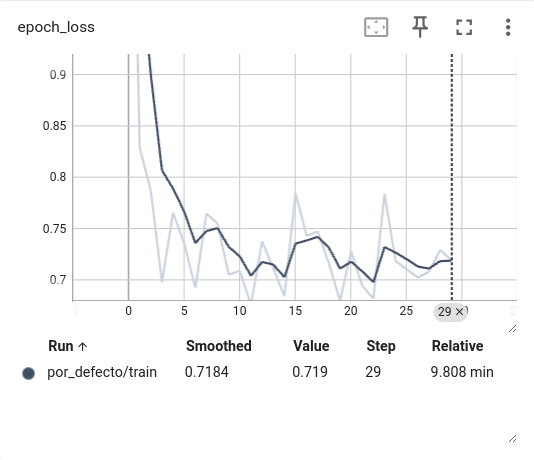
\includegraphics[scale=0.4]{plantilla-libro/img/loss.png}
\end{minipage}
\begin{minipage}[f]{0.5\textwidth}
  \centering 
  Capas De Clasificación \\
  \vspace{0.1cm}
  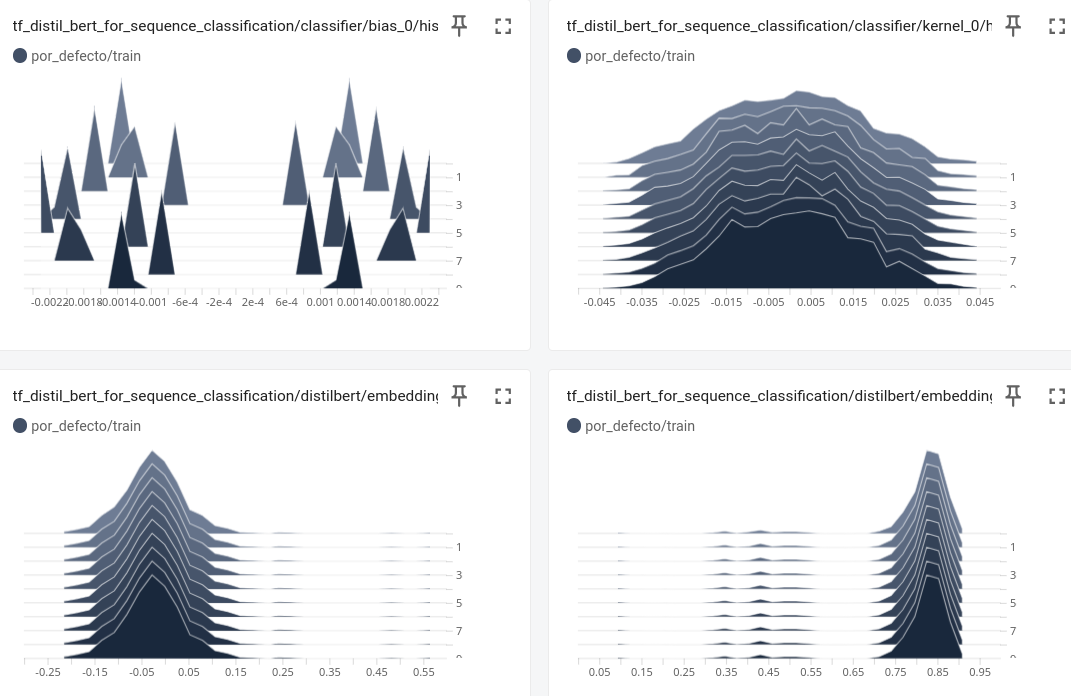
\includegraphics[scale=0.24]{plantilla-libro/img/capas.png}  
\end{minipage}


  % \centering

  \caption{(izquierda) Pérdida por epoca. (derecha) Capas de clasificación del modelo ajuadado. Fuente: Elaboración propia}
  \label{fig:ajuste-practico}
\end{figure}
      \end{enumerate}
      

       
\section{Futuro de los Modelos de Lenguaje Grandes}
   Las tendencias emergentes en la investigación y desarrollo de modelos de lenguaje grandes \cite{Shaip-LLM} incluyen avances hacia modelos aún más grandes y complejos que puedan capturar y generar un entendimiento más profundo del lenguaje natural. Se espera que los modelos futuros mejoren en áreas como la comprensión contextual, la generación de texto creativo y la adaptación a tareas especializadas.

   Los desafíos y consideraciones éticas en el uso de modelos de lenguaje a gran escala son significativos. Esto incluye preocupaciones sobre la privacidad y la seguridad de los datos utilizados para entrenar estos modelos, así como el sesgo y la equidad en las aplicaciones de IA que pueden afectar a diferentes grupos de manera desproporcionada. Otros aspectos éticos incluyen el uso responsable de la tecnología, la transparencia en los procesos de desarrollo y la regulación para garantizar un uso ético y seguro de los modelos de lenguaje grandes en diversos contextos sociales y empresariales.
\section{Conclusiones}

Los modelos de lenguaje grandes son uno de los avances más revolucionarios de los últimos años, cuyo desarrollo está en auge y se prevé que cambie el mundo tecnológico. En el pasado, las redes neuronales recurrentes tenían limitaciones a la hora de recordar el contexto, estas fueron actualizadas con capas de atención pero no fue hasta la aparición de los transformers en el articulo Attentión is all you need \cite{vaswani2023attention} que se impulsó la creación de modelos cada vez más eficientes y consecuentemente más grandes. El campo de la salud está en una fase prematura debido a las limitaciones burocráticas pero están saliendo a la luz proyectos que prometen cambiar la medicina en el largo plazo como MAPIC \cite{UMA}. En el documento se explican los mecanimos y arquitecturas que conforman estos modelos como los embedings, positional encodings y capas de atención. También se recoge un ejemplo de implementación de ajuste fino de BERT donde se cuentan los puntos claves y aspectos a tener en cuenta.

\listoffigures

\bibliography{biblio2}






